\documentclass{standalone}

\usepackage{tikz}
    \usetikzlibrary{arrows.meta}
    \usetikzlibrary{calc}
    \usetikzlibrary{decorations.pathmorphing}
    
\begin{document}
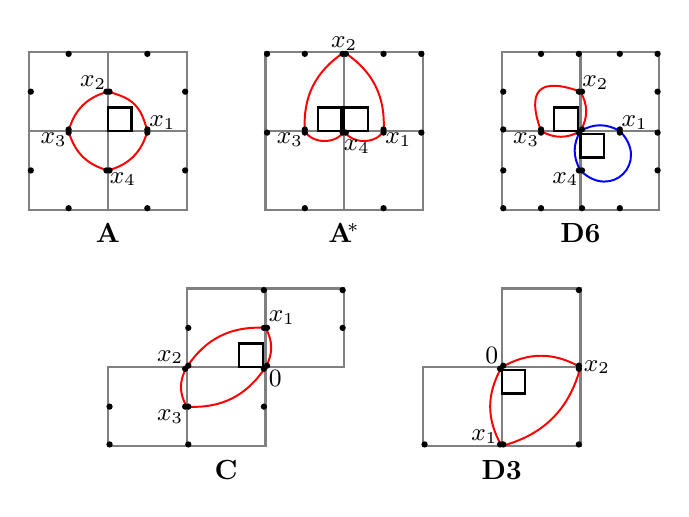
\begin{tikzpicture}
    % \draw[help lines] (0,0) grid (15,3);
    \foreach \x in % green
        {(0,0), (0,1), (1,0), (1,1),
         (3,0), (4,0), (3,1), (4,1), 
         (6,0), (7,0), (6,1), (7,1),
         (1,-3), (2,-3), (2,-2), (3,-2),
         (5,-3), (6,-3), (6,-2)} 
        {\draw[black!50, line width=0.3mm] \x rectangle+(1,1);}
    \foreach \x in % green
        {(1,1), (4,1), (3.666,1), (7,0.666), (6.666,1), (2.666,-2), (6,-2.333)} 
        {\draw[black, line width=0.3mm] \x rectangle+(0.3,0.3);}
    \path[line width=0.25mm]
        (1,0.5) edge[red, bend right] (1.5,1)
        (1.5,1) edge[red, bend right, looseness=1.2] (1,1.5)
        (1,1.5) edge[red, bend right] (0.5,1)
        (0.5,1) edge[red, bend right] (1,0.5)
        (4.5,1) edge[red, bend right] (4,2)
        (4,2) edge[red, bend right] (3.5,1)
        (3.5,1) edge[red, bend right=60] (4,1)
        (4,1) edge[red, bend right=60] (4.5,1)
        (7,1) edge[red, bend right] (7,1.5)
        (7,1.5) edge[red, in=110, out=160, looseness=2] (6.5,1)
        (6.5,1) edge[red, bend right] (7,1)
        (7,1) edge[blue, bend left] (7.5,1)
        (7.5,1) edge[blue, in=315, out=315, looseness=2] (7,0.5)
        (7,0.5) edge[blue, bend left] (7,1)
        (3,-2) edge[red, bend right] (3,-1.5)
        (3,-1.5) edge[red, bend right] (2,-2)
        (2,-2) edge[red, bend right] (2,-2.5)
        (2,-2.5) edge[red, bend right] (3,-2)
        (6,-3) edge[red, bend right] (7,-2)
        (7,-2) edge[red, bend right] (6,-2)
        (6,-2) edge[red, bend right] (6,-3);
    % case (A)1 bound
    \foreach \x in
        {(0,0), (0,1), (1,0), (1,1)} 
        {\fill \x++(0.02,0.5) circle (0.04);
         \fill \x++(0.98,0.5) circle (0.04);
         \fill \x++(0.5,0.02) circle (0.04);
         \fill \x++(0.5,0.98) circle (0.04);}
    % case (A)2 bound
    \foreach \x in
        {(3,0), (4,0), (3,1), (4,1)} 
        {\fill \x++(0.02,0.98) circle (0.04);
         \fill \x++(0.98,0.98) circle (0.04);
         \fill \x++(0.5,0.02) circle (0.04);
         \fill \x++(0.5,0.98) circle (0.04);}
    % case (C) bound
    \foreach \x in
        {(1,-3), (2,-3), (2,-2), (3,-2)} 
        {\fill \x++(0.02,0.5) circle (0.04);
         \fill \x++(0.98,0.5) circle (0.04);
         \fill \x++(0.02,0.02) circle (0.04);
         \fill \x++(0.98,0.98) circle (0.04);}
    % case (D6) bound
    \foreach \x in
        {(6,0), (7,0), (6,1), (7,1)} 
        {\fill \x++(0.02,0.5) circle (0.04);
         \fill \x++(0.98,0.5) circle (0.04);
         \fill \x++(0.5,0.02) circle (0.04);
         \fill \x++(0.5,0.98) circle (0.04);
         \fill \x++(0.02,0.02) circle (0.04);
         \fill \x++(0.98,0.98) circle (0.04);}
    % case (D6) bound
    \foreach \x in
        {(5,-3), (6,-3), (6,-2)} 
        {\fill \x++(0.02,0.02) circle (0.04);
         \fill \x++(0.98,0.98) circle (0.04);
         \fill \x++(0.98,0.02) circle (0.04);}
    \node[above right=-1mm] at (1.5,1) {\small$x_1$};
    \node[above left=-1mm] at (1,1.5) {\small$x_2$};
    \node[below left=-1mm] at (0.5,1) {\small$x_3$};
    \node[below right=-1mm] at (1,0.5) {\small$x_4$};
    \node[below right=-1mm] at (4.5,1) {\small$x_1$};
    \node[above=-1mm] at (4,2) {\small$x_2$};
    \node[below left=-1mm] at (3.5,1) {\small$x_3$};
    \node[shift={(0.16,-0.2)}] at (4,1) {\small$x_4$};
    \node[above right=-1mm] at (7.5,1) {\small$x_1$};
    \node[above right=-1mm] at (7,1.5) {\small$x_2$};
    \node[below left=-1mm] at (6.5,1) {\small$x_3$};
    \node[below left=-1mm] at (7,0.5) {\small$x_4$};
    % \node[above left=-0.8mm] at (7,1) {\small$0$};
    \node[below right=-0.8mm] at (3,-2) {\small$0$};
    \node[above right=-0.8mm] at (3,-1.5) {\small$x_1$};
    \node[above left=-0.8mm] at (2,-2) {\small$x_2$};
    \node[below left=-0.8mm] at (2,-2.5) {\small$x_3$};
    \node[above left=-0.8mm] at (6,-2) {\small$0$};
    \node[shift={(-0.22,0.12)}] at (6,-3) {\small$x_1$};
    \node[right=-0.8mm] at (7,-2) {\small$x_2$};
    \node at (1,-0.3) {\textbf{A}};
    \node at (4,-0.3) {\textbf{A\!}$^*$};
    \node at (7,-0.3) {\textbf{D6}};
    \node at (2.5,-3.3) {\textbf{C}};
    \node at (6,-3.3) {\textbf{D3}};
\end{tikzpicture}
\end{document}